\chapter{Developmental Genetics and Evolution of Form}\label{ch:b3:developmental-genetics}

A fruit fly's egg is half a millimetre long, and in the three hours
after fertilisation, before a single cell membrane has formed between
its six thousand nuclei, it decides which end will be the head, which
the tail, where each of fourteen segments will lie, and which of them
will carry legs, wings or antennae. It does so with a few dozen genes,
turned on in a hierarchy of ever finer stripes, each stripe read from
the concentrations of the products of the stripes before it. In 1980
two young scientists in Heidelberg screened thousands of mutant flies
for larvae with missing or duplicated parts, and found the whole
hierarchy: genes whose loss deletes a block of segments, genes whose
loss deletes every other segment, genes whose loss turns every segment
back to front. The same year's work on a gene that turns a fly's third
segment into a copy of its second --- giving it four wings, as its
ancestors had --- opened a set of master genes that, it turned out,
lay in the same order along the chromosomes of a mouse and a human,
and did the same job. This chapter is about how an embryo computes its
own geometry, how a few hundred regulatory genes build every animal
body, and how changing when and where they act has produced the
diversity of animal form.

\section{The fly's coordinates}

\begin{definition}[The segmentation hierarchy]\label{def:b3:developmental-genetics:hierarchy}
\index{maternal effect gene}\index{gap gene}\index{pair-rule gene}\index{segment polarity gene}\index{syncytial blastoderm}
The \emph{Drosophila} embryo develops for its first thirteen nuclear
divisions as a \emph{syncytial blastoderm}, a single cell whose nuclei
share one cytoplasm, so that proteins diffuse freely from where they are
made. Four gradients laid down by the mother's cells set the axes:
\emph{bicoid} mRNA is tethered at the anterior pole and its protein
diffuses back to form an exponential gradient from head to tail;
\emph{nanos} mRNA at the posterior pole makes the mirror gradient;
\emph{hunchback} and \emph{caudal} mRNAs are uniform, but Bicoid
protein represses \emph{caudal} translation and Nanos represses
\emph{hunchback}, so their proteins form gradients too. These
\emph{maternal-effect} products, whose mutant phenotype depends on the
mother's genotype and not the embryo's, switch on the \emph{gap genes}
(\emph{hunchback}, \emph{Kr{\"u}ppel}, \emph{knirps}, \emph{giant}) in
broad bands, each responding to a range of Bicoid concentration and
repressing its neighbours; the gap proteins, in combination, switch on
the \emph{pair-rule genes} (\emph{even-skipped}, \emph{fushi tarazu},
\emph{hairy}) in seven stripes each, alternating; and the pair-rule
proteins switch on the \emph{segment polarity genes} (\emph{engrailed},
\emph{wingless}, \emph{hedgehog}) in fourteen stripes, one per segment,
which fix each segment's front and back and are maintained, after the
cells form, by signalling between them. Three hours, four tiers, from a
single gradient to fourteen segments --- and the mutant names record
the screen: \emph{hunchback} lacks the thorax, \emph{Kr{\"u}ppel} (``cripple'')
the middle, \emph{fushi tarazu} (``not enough segments'') every other
segment, \emph{hedgehog} has a lawn of bristles.
\end{definition}

\begin{omfigure}
\begin{tikzpicture}[every node/.style={font=\scriptsize}, >=stealth]
  \foreach \y/\lab/\n in {0/{maternal: Bicoid gradient}/1, -1.3/{gap genes: 4 broad bands}/2, -2.6/{pair-rule genes: 7 stripes}/3, -3.9/{segment polarity: 14 stripes}/4} {
    \draw[thick, gray!60] (0,\y) ellipse (3.6 and 0.5);
    \node[left, align=right] at (-3.8,\y) {\lab};
  }
  % bicoid gradient shading
  \begin{scope}
    \clip (0,0) ellipse (3.6 and 0.5);
    \shade[left color=omDef!80, right color=omDef!2] (-3.6,-0.5) rectangle (3.6,0.5);
  \end{scope}
  \node[right, font=\tiny] at (3.7,0) {anterior high};
  % gap bands
  \begin{scope}
    \clip (0,-1.3) ellipse (3.6 and 0.5);
    \fill[omDef!50] (-3.4,-1.8) rectangle (-1.6,-0.8); \fill[omThm!40] (-1.4,-1.8) rectangle (0.2,-0.8); \fill[omMeth!40] (0.4,-1.8) rectangle (1.7,-0.8); \fill[omProp!45] (1.9,-1.8) rectangle (3.4,-0.8);
  \end{scope}
  \node[font=\tiny] at (-2.5,-1.3) {\emph{hb}}; \node[font=\tiny] at (-0.6,-1.3) {\emph{Kr}}; \node[font=\tiny] at (1.05,-1.3) {\emph{kni}}; \node[font=\tiny] at (2.65,-1.3) {\emph{gt}};
  % pair-rule stripes
  \begin{scope}
    \clip (0,-2.6) ellipse (3.6 and 0.5);
    \foreach \i in {0,...,6} { \fill[omThm!50] ({-3.1+\i*0.9},-3.1) rectangle ({-2.75+\i*0.9},-2.1); }
  \end{scope}
  \node[right, font=\tiny] at (3.7,-2.6) {\emph{eve}, every other segment};
  % segment polarity stripes
  \begin{scope}
    \clip (0,-3.9) ellipse (3.6 and 0.5);
    \foreach \i in {0,...,13} { \fill[omProp!60] ({-3.25+\i*0.47},-4.4) rectangle ({-3.1+\i*0.47},-3.4); }
  \end{scope}
  \node[right, font=\tiny] at (3.7,-3.9) {\emph{en}: one per segment};
  \foreach \y in {-0.55,-1.85,-3.15} { \draw[->, thick] (0,\y) -- (0,\y-0.2); }
  \node[below, align=center, font=\tiny] at (0,-4.5) {each tier reads the concentrations of the tier above;\\three hours from a single gradient to fourteen segments};
\end{tikzpicture}

{\small The segmentation hierarchy. A maternal gradient is read into
four gap-gene bands; the gap proteins, in combination, into seven
pair-rule stripes; those into fourteen segment-polarity stripes. Each
stripe is a boundary drawn where a concentration crosses a threshold.}
\end{omfigure}

\begin{theorem}[A morphogen gradient from synthesis, diffusion and decay]\label{thm:b3:developmental-genetics:gradient}
\index{morphogen}\index{positional information}\index{French flag model}\index{decay length}
A protein made at one end of a tissue at rate $J$ (per unit area),
diffusing with coefficient $D$ and degraded with rate constant $k$,
reaches a steady state in which its concentration along the axis $x$
obeys
\[
D\,\frac{\mathrm{d}^{2}c}{\mathrm{d}x^{2}} - k\,c = 0,
\qquad c(x) = c_{0}\,\mathrm{e}^{-x/\lambda}, \qquad \lambda = \sqrt{D/k},
\quad c_{0} = \frac{J}{\sqrt{Dk}} .
\]
The \emph{\omterm{thm:b3:developmental-genetics:gradient}{decay length}} $\lambda$ sets the gradient's reach; a cell
reads its position by comparing $c$ with thresholds --- the
\emph{French flag} of Wolpert (1969): above $T_{1}$ blue, between
$T_{1}$ and $T_{2}$ white, below red --- and the boundary for threshold
$T$ lies at $x_{T} = \lambda\ln(c_{0}/T)$. Two consequences: doubling
the source shifts every boundary back by the same $\lambda\ln 2$, and a
fractional error $\delta c/c$ in reading the concentration is a
positional error $\delta x = \lambda\,\delta c/c$, so a gradient can
place a boundary to within one cell only if the cells read it to within
a few per cent. Bicoid has $\lambda \approx \qty{100}{\micro m}$ in an
egg of \qty{500}{\micro m}: the gradient spans a factor $\mathrm{e}^{5}
\approx 150$, and the \emph{hunchback} boundary sits at mid-egg where
Bicoid has fallen to about a twelfth of its peak.
\end{theorem}
\begin{proof}
Conservation in a slab between $x$ and $x + \mathrm{d}x$: the net
diffusive inflow $D\,\partial^{2}c/\partial x^{2}$ balances the
degradation $kc$ at steady state, giving the equation; the solution
bounded as $x \to \infty$ is the decaying exponential with
$\lambda^{2} = D/k$. The source: the diffusive flux at $x = 0$, $-D\,
c'(0) = Dc_{0}/\lambda$, equals $J$, so $c_{0} = J\lambda/D =
J/\sqrt{Dk}$. Threshold: $c_{0}\mathrm{e}^{-x_{T}/\lambda} = T$ gives
$x_{T}$; doubling $c_{0}$ adds $\lambda\ln 2$ to every $x_{T}$
regardless of $T$. Error: differentiating $x_{T} = \lambda\ln(c_{0}/c)$,
$\delta x = -\lambda\,\delta c/c$. The steady state is reached on the
time scale $1/k$, which for Bicoid (\qty{50}{min}) is comparable to the
two hours available, so the gradient is read while still settling.
\end{proof}

\begin{omfigure}
\begin{tikzpicture}
\begin{axis}[
  width=0.7\linewidth, height=5.6cm,
  axis x line=bottom, axis y line=left,
  xmin=0, xmax=500, ymin=0, ymax=1.05,
  xlabel={distance from the anterior pole (\unit{\micro m})}, ylabel={Bicoid, relative},
  xlabel style={font=\small, at={(axis description cs:0.5,-0.12)}, anchor=north}, ylabel style={font=\small},
  tick label style={font=\small}, xtick={0,100,250,400,500}, ytick={0.08,0.3,0.6,1},
  yticklabels={0.08,0.3,0.6,1},
  clip=false,
]
\fill[omDef!15] (axis cs:0,0) rectangle (axis cs:120,1.05);
\fill[gray!8] (axis cs:120,0) rectangle (axis cs:250,1.05);
\fill[omThm!12] (axis cs:250,0) rectangle (axis cs:500,1.05);
\addplot[very thick, omDef, domain=0:500, samples=100] {exp(-x/100)};
\addplot[thick, omDef!50, dashed, domain=66:500, samples=100] {2*exp(-x/100)};
\draw[dashed, gray] (axis cs:0,0.3) -- (axis cs:120,0.3) -- (axis cs:120,0);
\draw[dashed, gray] (axis cs:0,0.08) -- (axis cs:250,0.08) -- (axis cs:250,0);
\node[font=\scriptsize, anchor=south] at (axis cs:60,1.0) {head};
\node[font=\scriptsize, anchor=south] at (axis cs:185,1.0) {thorax};
\node[font=\scriptsize, anchor=south] at (axis cs:375,1.0) {abdomen};
\node[font=\scriptsize, omDef, anchor=west] at (axis cs:255,0.35) {$c = c_{0}\,\mathrm{e}^{-x/\lambda}$, $\lambda = \qty{100}{\micro m}$};
\node[font=\scriptsize, omDef!70!black, anchor=west, align=left] at (axis cs:255,0.62) {dashed: source doubled ---\\every boundary shifts by $\lambda\ln 2 = \qty{69}{\micro m}$};
\node[font=\scriptsize, gray, anchor=north east] at (axis cs:118,0.29) {$T_{1}$};
\node[font=\scriptsize, gray, anchor=south west] at (axis cs:300,0.09) {$T_{2}$: \emph{hunchback} off};
\end{axis}
\end{tikzpicture}

{\small The French flag drawn by an exponential. Thresholds on one
gradient partition the egg into regions; a stronger source moves all
the boundaries backward by the same distance, which is what embryos
from mothers with extra copies of \emph{bicoid} show.}
\end{omfigure}

\begin{proof}[Evidence]
Nüsslein-Volhard and Wieschaus (1980) fed flies a mutagen, bred the
descendants to homozygosity, and looked at the cuticles of some
\num{27000} dead larvae under the microscope for missing or repeated
pattern: about a hundred and twenty genes, sorted by their phenotypes
into the gap, pair-rule and segment-polarity classes --- a hierarchy
visible before any molecule was known. Driever and Nüsslein-Volhard
(1988) stained embryos for Bicoid protein and saw the exponential
gradient from the anterior pole; embryos from mothers with one, two,
four or six copies of the gene had gradients of proportionate height,
and the head fold and the \emph{hunchback} boundary moved posteriorly
with the dose, as the threshold model predicts and by roughly the
$\lambda\ln 2$ per doubling it requires. Injecting \emph{bicoid} mRNA
into the middle of an egg produced a head there.
\end{proof}

\begin{omfigure}
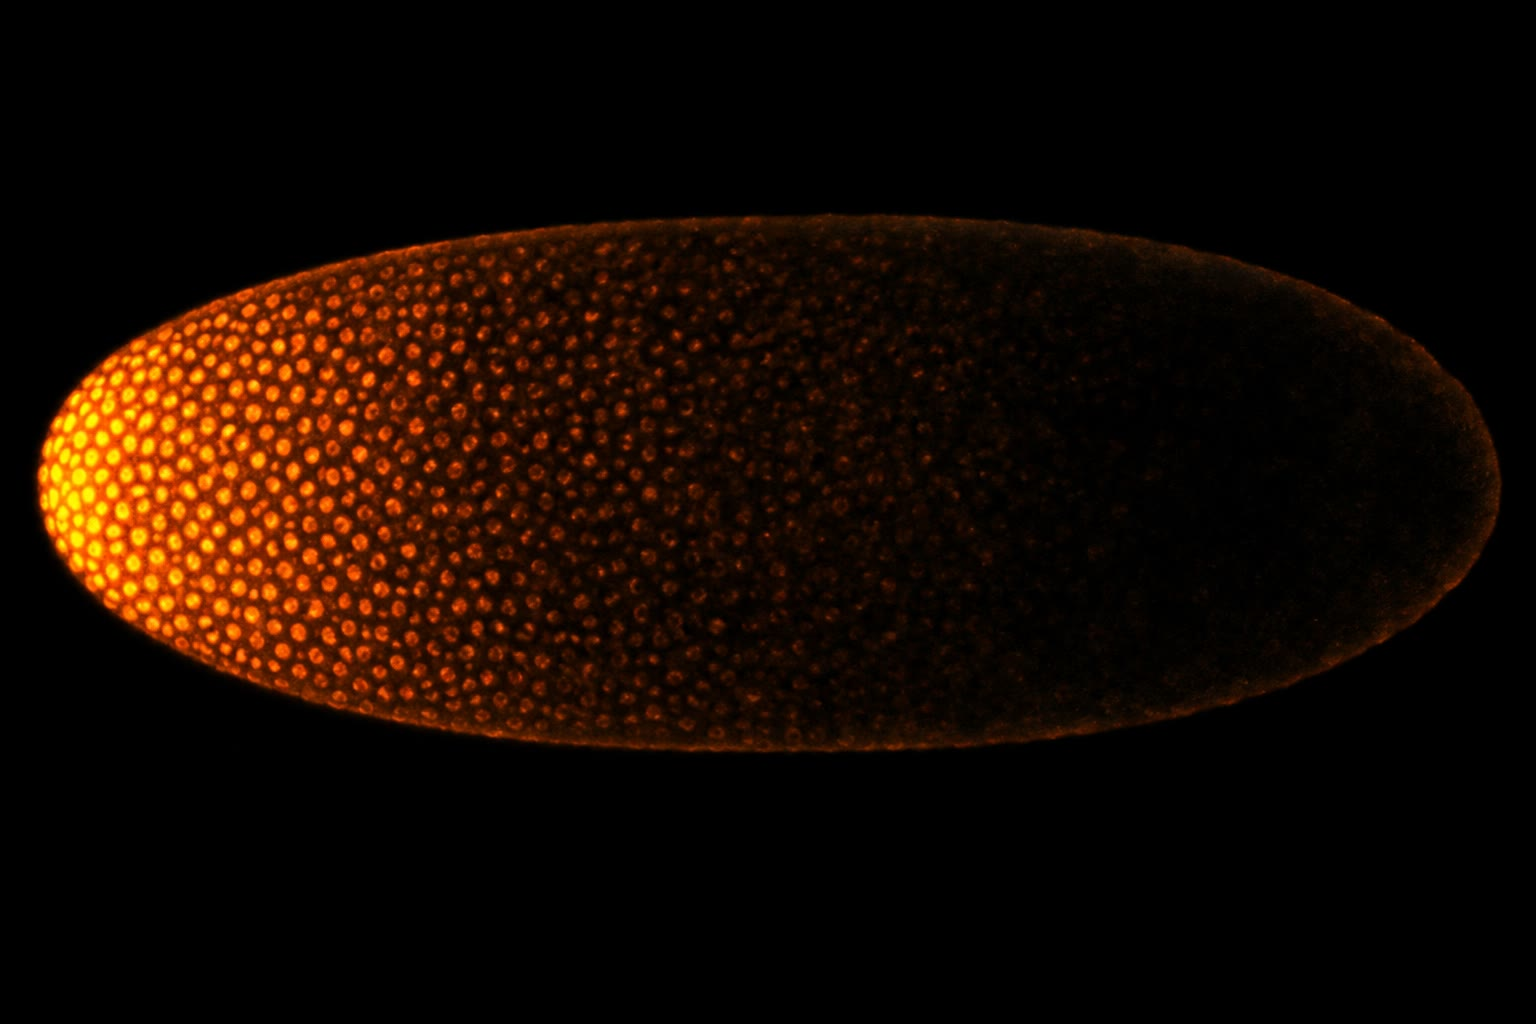
\includegraphics[width=0.46\linewidth]{images/book5/ai/b5-23-bicoid-gradient.jpg}\hspace{0.04\linewidth}
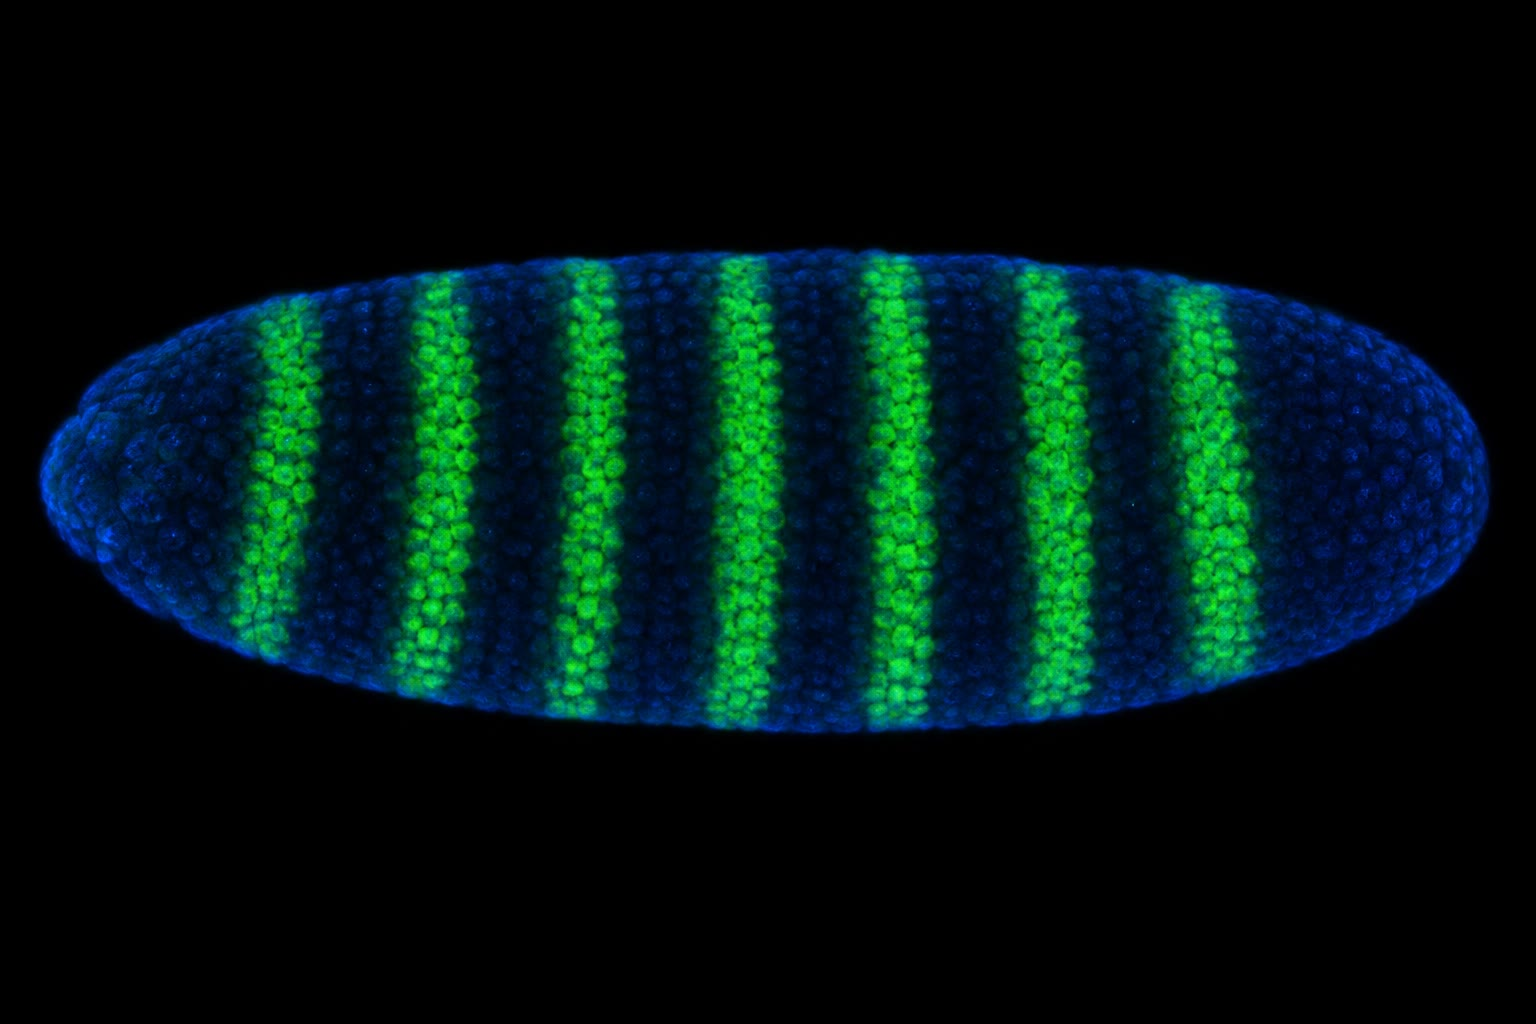
\includegraphics[width=0.46\linewidth]{images/book5/ai/b5-23-embryo-stripes.jpg}

{\small Left: a syncytial embryo stained for Bicoid protein, brightest
at the anterior pole and fading exponentially toward the posterior.
Right: an embryo an hour later stained for a pair-rule protein, seven
stripes drawn from the gap-gene bands.}
\end{omfigure}

\section{Identity: the Hox genes}

\begin{definition}[Homeotic genes and colinearity]\label{def:b3:developmental-genetics:hox}
\index{homeotic mutation}\index{Hox genes}\index{colinearity}\index{homeobox}\index{Hox code}
A \emph{homeotic} mutation turns one body part into another:
Bateson's word (1894) for the abnormalities that ``substitute one
member of a series for another.'' In the fly, \emph{Antennapedia}
dominant mutants grow legs where antennae should be; \emph{bithorax}
mutants (Lewis, 1978) turn the third thoracic segment into a copy of
the second, so that the balancers (halteres) become a second pair of
wings. The eight genes responsible, the \emph{Hox genes}, lie in two
clusters on one chromosome, and Lewis noticed that their order along
the DNA matches the order along the body of the segments they control
--- \emph{colinearity}, still not fully explained. Each encodes a
transcription factor with the same 60-amino-acid DNA-binding
\emph{homeobox} domain (McGinnis, Gehring, 1984), which was then found
in every animal: mice and humans carry four clusters of thirteen genes
each, colinear in the same way, expressed in nested domains along the
body axis, the later genes in the cluster more posterior. A cell's
identity along the axis is given by the combination of Hox genes it
expresses, the \emph{Hox code}; posterior genes dominate anterior ones
(posterior prevalence), so losing a posterior gene lets the segment
adopt the identity of the one in front. Hox genes do not build a
segment; they tell an already-built segment which one it is, by
switching on the batteries of downstream genes appropriate to a leg, a
wing, a rib or a lumbar vertebra.
\end{definition}

\begin{omfigure}
\begin{tikzpicture}[every node/.style={font=\scriptsize}, >=stealth]
  % fly cluster
  \node[left] at (-0.3,2.2) {fly (\emph{Drosophila}), 8 genes};
  \foreach \i/\g/\c in {0/lab/omDef, 1/pb/omDef, 2/Dfd/omThm, 3/Scr/omThm, 4/Antp/omMeth, 5/Ubx/omMeth, 6/abd-A/omProp, 7/Abd-B/omProp} {
    \draw[thick, fill=\c!40] ({\i*1.1},1.9) rectangle ({\i*1.1+0.9},2.5); \node[font=\tiny] at ({\i*1.1+0.45},2.2) {\emph{\g}};
  }
  \node[left] at (-0.3,0.9) {mouse HoxB cluster, 9 of 13};
  \foreach \i/\g/\c in {0/b1/omDef, 1/b2/omDef, 2/b3/omDef, 3/b4/omThm, 4/b5/omThm, 5/b6/omMeth, 6/b7/omMeth, 7/b8/omProp, 8/b9/omProp} {
    \draw[thick, fill=\c!40] ({\i*1.1},0.6) rectangle ({\i*1.1+0.9},1.2); \node[font=\tiny] at ({\i*1.1+0.45},0.9) {\emph{\g}};
  }
  \draw[->, thick] (0,1.55) -- (9.8,1.55); \node[above, font=\tiny] at (4.9,2.55) {3$'$ $\to$ 5$'$ along the DNA};
  \draw[->, thick] (0,0.2) -- (9.8,0.2); \node[below, font=\tiny] at (4.9,0.05) {anterior $\to$ posterior along the body};
  % body schematic
  \node[left] at (-0.3,-0.9) {expressed in};
  \draw[thick, gray!70, rounded corners=6pt] (0,-1.3) rectangle (9.8,-0.5);
  \foreach \x/\t in {0.6/head, 2.6/neck, 4.4/thorax, 6.6/lumbar, 8.6/{sacral, tail}} { \node[font=\tiny] at (\x,-0.9) {\t}; }
  \draw[gray!70] (1.6,-1.3) -- (1.6,-0.5); \draw[gray!70] (3.5,-1.3) -- (3.5,-0.5); \draw[gray!70] (5.6,-1.3) -- (5.6,-0.5); \draw[gray!70] (7.6,-1.3) -- (7.6,-0.5);
  \node[below, align=center, font=\tiny] at (4.9,-1.4) {colinearity: the order of the genes on the chromosome is the order of their domains along the body;\\the same clusters, the same order, from fly to mouse ---\\inherited from an ancestor 600 million years ago};
\end{tikzpicture}

{\small Hox clusters in a fly and a mouse. The genes lie along the DNA in
the order of the body regions they specify, in both animals, and the
homologous genes can be told by sequence: a mouse \emph{Hoxb6} gene is
recognisably the fly's \emph{Antennapedia}.}
\end{omfigure}

\begin{proof}[Evidence]
Lewis (1978) mapped the \emph{bithorax} complex as a series of
mutations each transforming one segment into the one in front, arranged
on the chromosome in body order, and proposed that the genes were
sequentially activated along the axis. McGinnis and colleagues (1984)
found the \omterm{def:b3:developmental-genetics:hox}{homeobox} by cross-hybridisation between \emph{Antennapedia}
and \emph{Ultrabithorax} and then in frogs and mice. The functional
equivalence was shown directly: a mouse \emph{Hoxb6} gene expressed in a
fly produces the \emph{Antennapedia} phenotype, legs from antennae
(1990s); a mouse lacking \emph{Hoxc8} has an extra rib on its first
lumbar vertebra, the segment having taken the identity of the one in
front; and altering Hox expression boundaries in chick and mouse shifts
the position where forelimbs form, the neck's length in a swan being
matched by a posterior shift of the same boundary.
\end{proof}

\begin{omfigure}
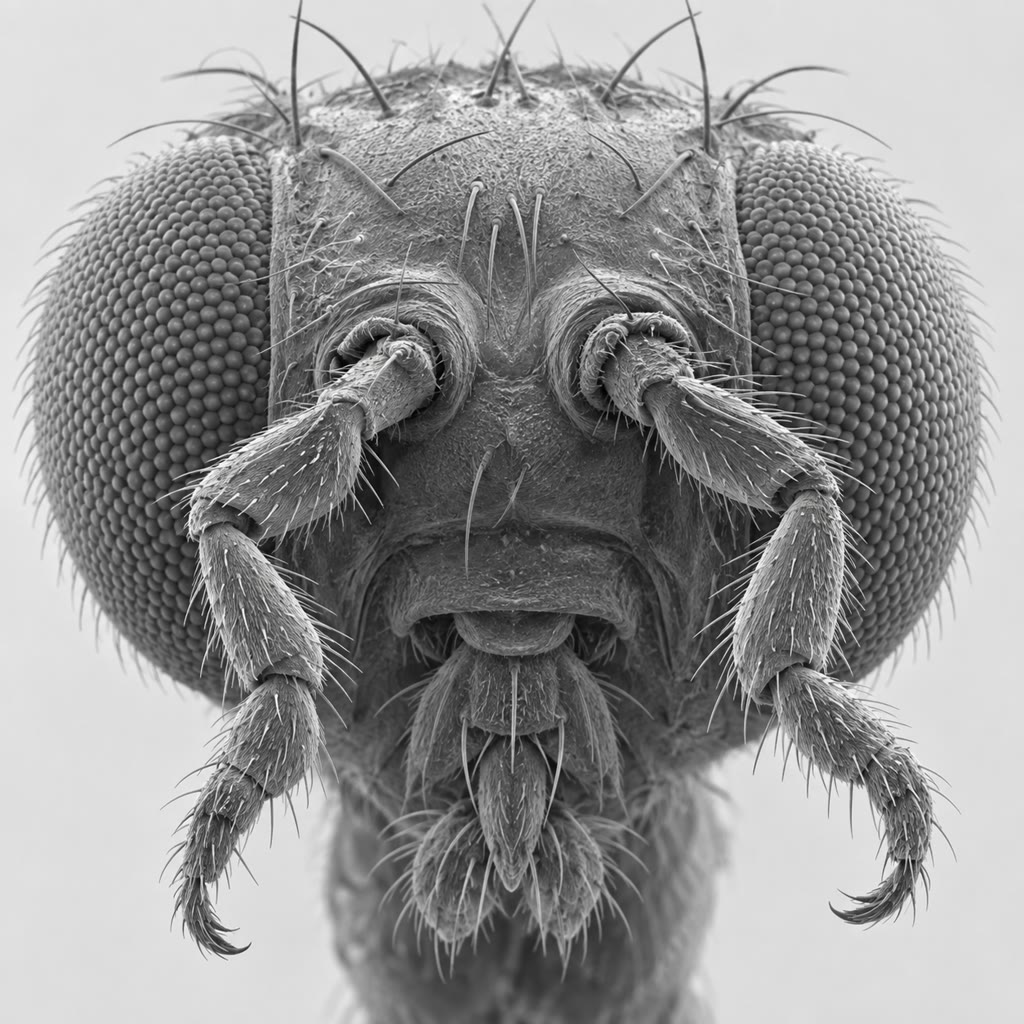
\includegraphics[width=0.34\linewidth]{images/book5/ai/b5-23-antennapedia-fly.jpg}\hspace{0.04\linewidth}
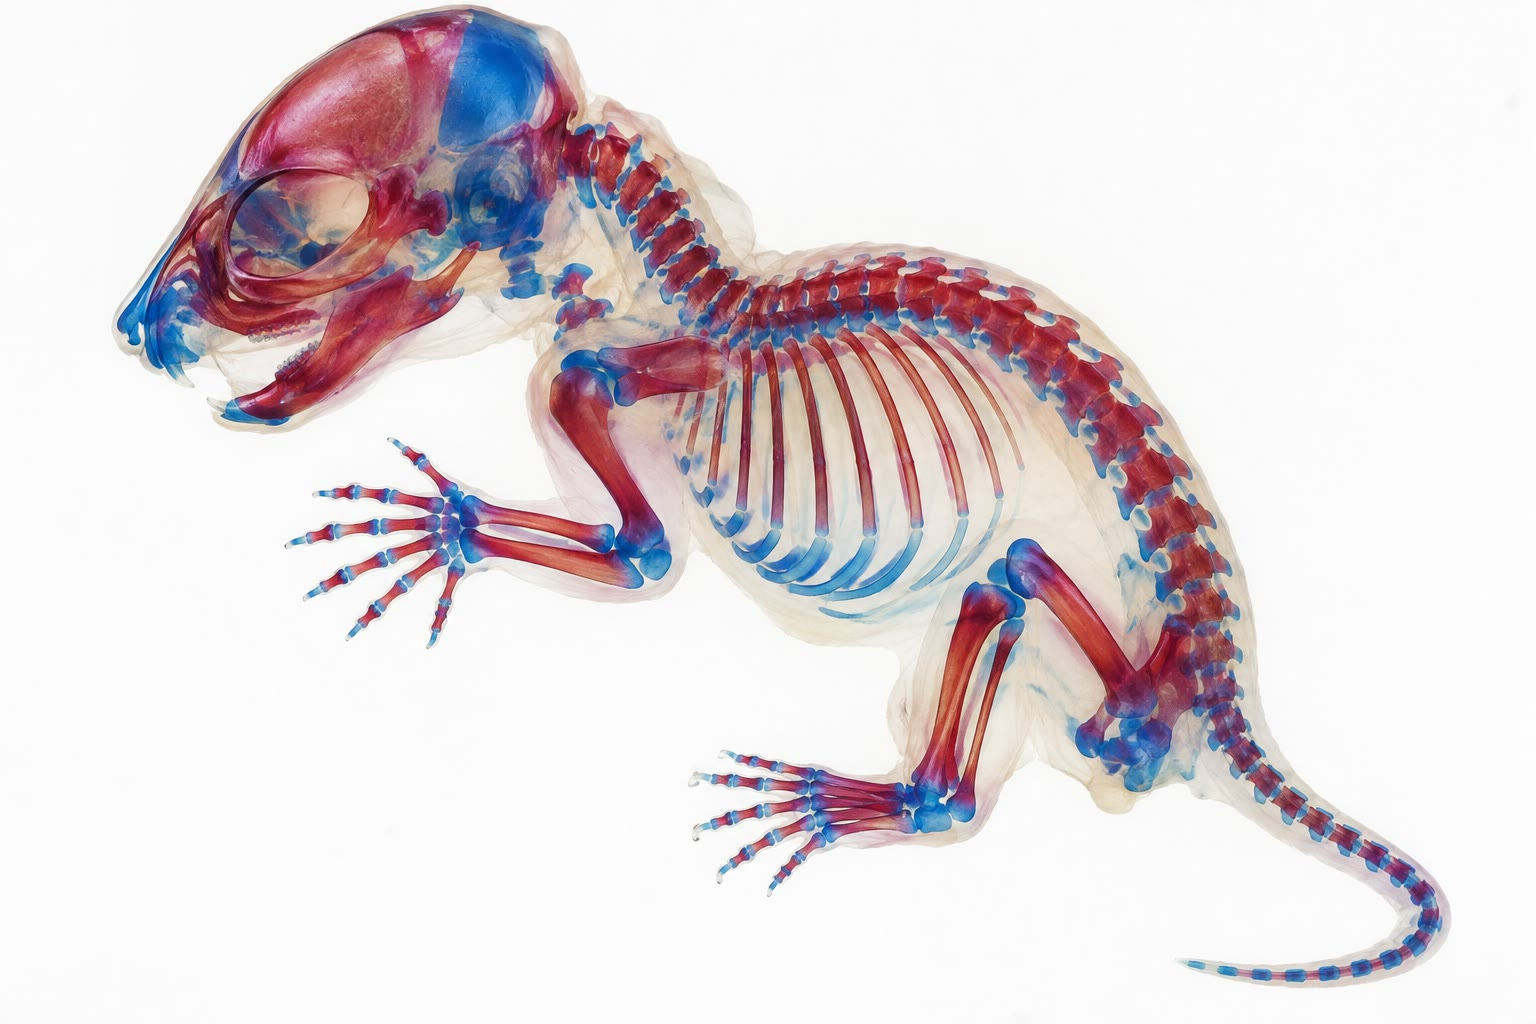
\includegraphics[width=0.5\linewidth]{images/book5/ai/b5-23-limb-skeleton-stain.jpg}

{\small Left: the head of an \emph{Antennapedia} mutant fly, a pair of
legs where the antennae should be --- the segment built correctly and
told the wrong identity. Right: a mouse embryo's skeleton, cartilage
blue and bone red, the vertebrae along which the \omterm{def:b3:developmental-genetics:hox}{Hox code} is read.}
\end{omfigure}

\section{Building a vertebrate}

\begin{definition}[Organisers and signalling centres]\label{def:b3:developmental-genetics:organiser}
\index{organiser}\index{induction}\index{sonic hedgehog}\index{limb bud}\index{zone of polarising activity}\index{apical ectodermal ridge}
Vertebrate embryos are cellular from the start, so their gradients are
made by secreted proteins rather than a syncytium's diffusion, and the
same few families do everything: Wnt, Hedgehog, BMP and other TGF-$\beta$
relatives, FGF, Notch and retinoic acid. Spemann and Mangold (1924)
grafted a piece of the dorsal lip of a newt gastrula onto the belly of
another and obtained a second embryo, head to tail, made mostly of host
cells: the graft was an \emph{organiser}, inducing its neighbours to
form a nervous system and axis, and its molecules were found seventy
years later to be secreted antagonists (Chordin, Noggin) that block
BMP, whose absence lets ectoderm become neural --- the default. The
\emph{neural tube} is then patterned dorsoventrally by \emph{sonic
hedgehog} from the notochord and floor plate (high: motor neurons; low:
\omterm{def:b3:nervous-systems:cells}{interneurons}) against BMP from the roof; and the \emph{limb bud} by two
centres, the \emph{zone of polarising activity} at its posterior margin
secreting Shh (its graft to the anterior margin gives a mirror-image
duplication of the digits, six fingers meeting thumb to thumb) and the
\emph{apical ectodermal ridge} at its tip secreting FGFs that keep the
underlying cells dividing and specify the proximal-to-distal sequence
of humerus, forearm, hand. Grafting, ablation and beads soaked in
protein remain the tools; the logic --- a local source, a gradient,
thresholds, a code of transcription factors --- is the fly's.
\end{definition}

\begin{omfigure}
\begin{tikzpicture}[every node/.style={font=\scriptsize}, >=stealth]
  % limb bud
  \fill[omDef!12] (0,0) -- (0,3) .. controls (2.6,3.4) and (3.4,2.2) .. (3.4,1.5) .. controls (3.4,0.8) and (2.6,-0.4) .. (0,0) -- cycle;
  \draw[thick, omDef] (0,0) -- (0,3) .. controls (2.6,3.4) and (3.4,2.2) .. (3.4,1.5) .. controls (3.4,0.8) and (2.6,-0.4) .. (0,0);
  \draw[very thick, omMeth!70!black] (2.9,2.5) .. controls (3.45,1.9) and (3.45,1.1) .. (2.9,0.5);
  \node[right, align=left, omMeth!70!black, font=\tiny] at (3.5,1.5) {apical ectodermal ridge:\\FGF8; keeps the\\progress zone dividing;\\proximal $\to$ distal};
  \begin{scope}
    \clip (0,0) -- (0,3) .. controls (2.6,3.4) and (3.4,2.2) .. (3.4,1.5) .. controls (3.4,0.8) and (2.6,-0.4) .. (0,0) -- cycle;
    \foreach \i/\op in {1/50, 2/38, 3/26, 4/14} { \draw[omThm!\op, thick] (0.6,0.5) circle ({0.45*\i}); }
  \end{scope}
  \fill[omThm!50] (0.6,0.5) ellipse (0.5 and 0.35); \node[anchor=north, align=center, omThm, font=\tiny] at (0.9,-0.2) {ZPA: sonic hedgehog,\\posterior $\to$ anterior};
  \node[left, font=\tiny] at (-0.05,2.6) {anterior}; \node[left, font=\tiny] at (-0.05,0.4) {posterior};
  \node[left, font=\tiny] at (-0.05,1.5) {body wall};
  \draw[->, thick] (0.3,1.5) -- (3.0,1.5); \node[above, font=\tiny] at (1.75,1.55) {humerus, forearm, digits};
  % right: digit code
  \node[right, align=left] at (7.2,2.6) {digit identity from Shh exposure:\\thumb (digit 1): none;\\digits 2--3: gradient;\\digits 4--5: from Shh-expressing cells};
  \node[right, align=left] at (7.2,1.0) {graft a second ZPA anteriorly:\\mirror-image duplication, 4-3-2-2-3-4;\\bead of Shh protein does the same};
  \node[right, align=left, gray] at (7.2,-0.2) {the same molecule patterns the neural tube\\(motor neurons where it is high) and the gut};
\end{tikzpicture}

{\small The \omterm{def:b3:developmental-genetics:organiser}{limb bud}'s two signalling centres. \omterm{def:b3:developmental-genetics:organiser}{Sonic hedgehog} from the
posterior margin tells cells which digit to become; FGF from the tip
tells them how far out along the limb they are. Grafts that move a
centre move the pattern with it.}
\end{omfigure}

\begin{proposition}[Spontaneous pattern: Turing's mechanism]\label{prop:b3:developmental-genetics:turing}
\index{Turing pattern}\index{reaction--diffusion}\index{activator--inhibitor}
Not every pattern is read from a pre-existing gradient. Turing (1952)
showed that two diffusing substances that react --- an \emph{activator}
that stimulates its own production and that of an \emph{inhibitor},
and an inhibitor that suppresses the activator and diffuses much
faster --- can turn a uniform field into a regular array of peaks
spontaneously: a small local excess of activator grows by
self-enhancement while the inhibitor it produces spreads out and
prevents new peaks forming nearby, so peaks appear at a spacing set by
the inhibitor's range, $\lambda \sim \sqrt{D_{\text{inh}}/k_{\text{inh}}}$,
and not by any external coordinate. The mechanism, admitted here in its
mathematics, is the best account of the spots and stripes of animal
coats, the spacing of hair follicles and feather buds, the ridges of
the palate, the digits of the hand (whose number rises when the
pattern's wavelength is shortened by lowering Hox activity), and the
stripes of zebrafish, where the interacting cells --- pigment cells
that repel neighbours of one kind and attract those of another at a
distance --- have been identified and their stripes made to re-form
after laser ablation exactly as the theory predicts.
\end{proposition}
\admitted

\section{Evolution of form}

\begin{definition}[Evo-devo]\label{def:b3:developmental-genetics:evodevo}
\index{deep homology}\index{genetic toolkit}\index{cis-regulatory evolution}\index{heterochrony}
The genes that build animals are an ancient and shared \emph{toolkit}:
a few hundred transcription factors and signalling pathways present
in the common ancestor of all animals, and animal diversity comes
mostly from changes in \emph{when, where and how much} they are
expressed rather than in what they encode. \emph{Deep homology}: the
gene \emph{Pax6} directs eye formation in flies, squid and mice, whose
eyes are not homologous as organs --- a mouse \emph{Pax6} expressed on a
fly's leg makes an ectopic fly eye there (Halder, Gehring, 1995).
\emph{Cis-regulatory evolution}: the loss of pelvic spines in
freshwater sticklebacks is the deletion of one enhancer of the
\emph{Pitx1} gene, the protein untouched and still serving elsewhere;
the loss of wing spots in some fruit flies, a change in an enhancer of
\emph{yellow}; the loss of legs in snakes, a broken enhancer of
\emph{\omterm{def:b3:developmental-genetics:organiser}{sonic hedgehog}} in the limb. \emph{Hox shifts}: the boundary of
\emph{Hoxc6} expression marks the first thoracic vertebra in mouse,
chick, goose and snake alike, at vertebra 7, 14, 23 and 3; insects'
loss of abdominal legs was the Hox protein Ubx acquiring a repressive
domain that switches off the leg gene \emph{Distal-less}, where in
crustaceans it does not. \emph{Heterochrony}, a change in the timing of
a developmental programme, made the axolotl a permanent larva and the
human face a juvenile ape's. The old question of how new forms arise
becomes a question about regulatory DNA: most of the genome that
matters for form is not gene but switch.
\end{definition}

\begin{example}[Four wings]\label{ex:b3:developmental-genetics:four-wings}
The ancestors of flies had four wings, as dragonflies and bees still
do; flies have two, the hind pair reduced to the balancers. In flies,
\emph{Ultrabithorax} is expressed in the third thoracic segment and
represses the wing programme there --- some hundred target genes, a
haltere being a wing with those genes switched off. Lewis's
triple-mutant fly, lacking \emph{Ubx} function in the third segment,
grows a second pair of wings: not a new structure but the release of
an old one. In butterflies \emph{Ubx} is expressed in the hindwing as
well, and there it does not suppress the wing but changes its pattern:
the same protein, a different set of targets. Four hundred million
years of dipteran evolution turned on one gene's decision in one
segment, and a single mutation undoes it in a generation --- which is
why the history of form is legible in the genes that build it.
\end{example}

\begin{remark}[Geometry from chemistry]\label{rem:b3:developmental-genetics:remark}
An embryo has no blueprint and no surveyor. It has a few gradients
made by diffusion and decay, cells that read them against thresholds
and switch on transcription factors, and a code of those factors that
tells each region what to become; it has local \omterm{def:b3:developmental-genetics:organiser}{organisers} that induce
their neighbours, and reactions that pattern themselves. The
mathematics is that of first-order kinetics and diffusion --- an
exponential, a square root, a threshold --- and it explains not only
how a fly's head is placed but why doubling a gene shifts a boundary
by a fixed distance, why six fingers appear when a signal is
duplicated, and why a snake has three hundred ribs. Evolution edits the
switches, not the machine: the toolkit of a sponge and a human is
nearly the same, and what differs is the wiring.
\end{remark}

\section{Exercises}

\begin{exercise}[$\star$]\label{exo:b3:developmental-genetics:1}
Name the four tiers of the fly's segmentation hierarchy, one gene of
each, and the mutant phenotype that placed it in its class.
\end{exercise}

\begin{exercise}[$\star$]\label{exo:b3:developmental-genetics:2}
What is a maternal-effect gene? A female homozygous for a \emph{bicoid}
null mutation is mated to a wild-type male: describe her embryos and
explain why their own genotype does not save them.
\end{exercise}

\begin{exercise}[$\star$]\label{exo:b3:developmental-genetics:3}
State \omterm{def:b3:developmental-genetics:hox}{colinearity} and posterior prevalence. Predict the phenotype of a
mouse lacking \emph{Hoxc8} and of a fly expressing \emph{Antennapedia}
in its head.
\end{exercise}

\begin{exercise}[$\star$]\label{exo:b3:developmental-genetics:4}
What did the Spemann--Mangold graft show, and what were the \omterm{def:b3:developmental-genetics:organiser}{organiser}'s
molecules found to be? Why is neural fate called the ``default''?
\end{exercise}

\begin{exercise}[$\star\star$]\label{exo:b3:developmental-genetics:5}
Bicoid: $D = \qty{4}{\micro m^2/s}$, half-life \qty{35}{min}. Compute
$k$, $\lambda$, and the ratio of concentrations at the anterior pole and
at mid-egg (\qty{250}{\micro m}).
\end{exercise}

\begin{exercise}[$\star\star$]\label{exo:b3:developmental-genetics:6}
With $\lambda = \qty{100}{\micro m}$, a boundary sits at
\qty{240}{\micro m}. Where does it sit if the mother carries four copies
of \emph{bicoid} instead of two? One copy? Express the shifts as a
fraction of a \qty{500}{\micro m} egg.
\end{exercise}

\begin{exercise}[$\star\star$]\label{exo:b3:developmental-genetics:7}
Nuclei at the blastoderm are \qty{8}{\micro m} apart. To place a
boundary to within one nucleus with $\lambda = \qty{100}{\micro m}$,
how precisely must a nucleus read the Bicoid concentration? If the
nucleus counts molecules over a time $\tau$ and the count is Poisson,
how many must it count?
\end{exercise}

\begin{exercise}[$\star\star$]\label{exo:b3:developmental-genetics:8}
The gradient approaches steady state on the time scale $1/k$. With a
half-life of \qty{35}{min}, what fraction of the steady-state
concentration is reached at \qty{60}{min}, \qty{90}{min} and
\qty{120}{min}? What does this imply for an embryo that must read the
gradient by \qty{150}{min}?
\end{exercise}

\begin{exercise}[$\star\star$]\label{exo:b3:developmental-genetics:9}
A ZPA is grafted to the anterior margin of a chick \omterm{def:b3:developmental-genetics:organiser}{limb bud}. Predict
the digit pattern, and the pattern if instead a bead releasing a low
dose of Shh is implanted there.
\end{exercise}

\begin{exercise}[$\star\star\star$]\label{exo:b3:developmental-genetics:10}
A morphogen is made throughout a tissue of length $L$ at rate $s$ per
unit volume, degraded at rate $k$, and destroyed at the boundary $x =
L$ (an absorbing sink), with no flux at $x = 0$. Solve $Dc'' - kc + s =
0$ for $c(x)$ and sketch it. How does this gradient's shape differ from
the source-at-one-end case, and what happens when $L \ll \lambda$?
\end{exercise}

\begin{exercise}[$\star\star\star$]\label{exo:b3:developmental-genetics:11}
Two thresholds at $T_{1} = 0.3c_{0}$ and $T_{2} = 0.08c_{0}$ divide a
gradient into three regions. Show that the widths of the first two
regions do not depend on $c_{0}$, and explain why an embryo whose
\emph{length} varies between individuals (\qty{450}{} to
\qty{550}{\micro m}) needs something more than a single exponential to
scale its pattern. Propose one mechanism.
\end{exercise}

\begin{exercise}[$\star\star\star$]\label{exo:b3:developmental-genetics:12}
Sticklebacks lost pelvic spines by deleting a \emph{Pitx1} enhancer,
snakes lost limbs by breaking a \emph{\omterm{def:b3:developmental-genetics:organiser}{sonic hedgehog}} enhancer. Explain
why regulatory changes rather than coding changes are the usual route
to a lost or altered structure, in terms of pleiotropy and of what the
same protein does elsewhere.
\end{exercise}

\section{Problem: The French Flag}

\begin{problem}[{Weekend problem --- an egg's coordinate system computed
from first-order kinetics: the Bicoid gradient's length, source and time
to form, the boundaries it draws and their precision, what gene dosage
and egg size do to them, and the Hox code read downstream, ending on the
decay length, the shift per doubling and the positional precision}]
\label{pb:b3:developmental-genetics:1}
Data: egg length \qty{500}{\micro m}; Bicoid $D = \qty{4}{\micro m^2/s}$,
half-life \qty{35}{min}; source flux such that $c_{0} = \qty{50}{nM}$
with two maternal copies; nuclear spacing \qty{8.5}{\micro m} at cycle
14; thresholds $T_{1} = 0.3\,c_{0}$ (head/thorax) and $T_{2} =
0.08\,c_{0}$ (\emph{hunchback} boundary) for the two-copy case. Read-out
noise $\delta c/c = 0.1$ for a single nucleus. Avogadro's number
\qty{6e23}{}; a nucleus is a sphere of radius \qty{3}{\micro m}.

\medskip
\noindent\textbf{Part I --- The gradient.}
\begin{enumerate}
  \item Compute $k$ from the half-life, in \unit{s^{-1}}, and the
        lifetime $1/k$ in minutes.
  \item Compute $\lambda = \sqrt{D/k}$ in micrometres. How many \omterm{thm:b3:developmental-genetics:gradient}{decay
        lengths} is the egg?
  \item The concentration falls by what factor from pole to pole? By
        what factor over one nuclear spacing at mid-egg?
  \item Compute the source flux $J = c_{0}\sqrt{Dk}$ in
        \unit{nM\,\micro m\,s^{-1}}, and the number of molecules
        entering a \qty{1}{\micro m^2} patch of the anterior pole per
        second.
  \item Number of Bicoid molecules in a nucleus at the pole ($c_{0}$)
        and at mid-egg.
  \item Fraction of the steady state reached at \qty{60}{min} and
        \qty{120}{min} ($1 - \mathrm{e}^{-kt}$). Is the gradient steady
        when the boundaries are drawn, at about \qty{120}{min}?
\end{enumerate}

\medskip
\noindent\textbf{Part II --- Boundaries.}
\begin{enumerate}[resume]
  \item Positions of the two boundaries, in \unit{\micro m} and as
        fractions of egg length.
  \item The mother has four copies: new $c_{0}$, and the two boundary
        positions. By how much did each move? Six copies?
  \item One copy: positions. Which regions grew, which shrank?
  \item Positional error from a \qty{10}{\%} read-out noise, in
        micrometres and in nuclear spacings.
  \item If the error must be one nucleus, what read-out precision is
        needed? If the nucleus averages over $n$ independent readings
        and the noise falls as $1/\sqrt{n}$, how many readings?
  \item A nucleus at the \emph{hunchback} boundary holds the number
        computed in question~5. What is the Poisson noise
        $1/\sqrt{N}$ of a single instantaneous count? Compare with
        \qty{10}{\%} and comment.
\end{enumerate}

\medskip
\noindent\textbf{Part III --- Scaling and robustness.}
\begin{enumerate}[resume]
  \item Eggs vary from \qty{450}{} to \qty{550}{\micro m}. If $\lambda$
        and $c_{0}$ are fixed, where does the \emph{hunchback} boundary
        fall as a fraction of egg length in each? Is the pattern scaled?
  \item Suppose instead that $D$ scales as $L^{2}$ (the same lifetime,
        but a source whose spread grows with the egg). Show that
        $\lambda/L$ is then constant and the pattern scales. Is this
        plausible?
  \item The \emph{hunchback} gene responds to Bicoid with a \omterm{def:b3:structural-biology:allostery}{Hill
        coefficient} of $5$: its expression is $c^{5}/(c^{5} + T^{5})$.
        Over how many micrometres does expression go from \qty{10}{\%}
        to \qty{90}{\%} around the boundary? Compare with one nuclear
        spacing.
  \item Explain why a steep response sharpens a boundary but does not
        by itself reduce the positional error due to concentration
        noise.
  \item Mutual repression between \omterm{def:b3:developmental-genetics:hierarchy}{gap genes} sharpens and stabilises
        their boundaries. Argue in a sentence why two genes that repress
        each other cannot both be on in the same nucleus at steady
        state.
  \item Temperature raises $D$ by \qty{2}{\%} and $k$ by \qty{6}{\%} per
        degree. Change in $\lambda$ per degree, and the boundary shift
        for a \qty{5}{\celsius} warmer room. Why might embryos need a
        compensating mechanism?
\end{enumerate}

\medskip
\noindent\textbf{Part IV --- Identity.}
\begin{enumerate}[resume]
  \item The \omterm{def:b3:developmental-genetics:hox}{Hox code}: with eight fly \omterm{def:b3:developmental-genetics:hox}{Hox genes} each on or off, how many
        codes are possible? How many are used (fourteen segments)? Why
        does posterior prevalence reduce the effective number?
  \item A fly lacks \emph{Ubx} in its third thoracic segment. What does
        the segment become, and why is the result four wings and not a
        new structure?
  \item A mouse's \emph{Hoxc6} boundary lies at vertebra 7, a goose's at
        23. What does this predict about their necks, and what changed
        in evolution: the gene, or its expression?
  \item A ZPA graft gives digits 4-3-2-2-3-4. Explain the pattern from
        two Shh gradients meeting in the middle.
  \item Halder and Gehring expressed mouse \emph{Pax6} in a fly's leg
        and obtained a fly eye there. What does this show about the
        gene, and what does it \emph{not} show about the eyes of flies
        and mice?
  \item The sixth finger: shortening Turing's wavelength adds a digit.
        With five digits across a \qty{2}{mm} hand plate, what
        wavelength change gives six? Which parameter of the
        reaction--diffusion system would produce it?
  \item Summarise: $\lambda$ (question~2), the boundary shift per
        doubling of the source (question~8), and the positional error
        from \qty{10}{\%} noise (question~10).
\end{enumerate}
\end{problem}
